%%%%%%%%%%%%%%%%%%
% 			 
%			Master Thesis - UWB
%				State of the art code
%
%			Author : Wilson Daubry
%
%%%%%%%%%%%%%%%%%%

\chapter{State of the art}
\label{stateoftheart}

This chapter outlines the state of the art. The first part focus on the implementation of a locating system, presented after a brief introduction to the \gls{uwb} and \gls{rtls}. Next, the concept of virtual anchors and multi-path aided locating systems is discussed.


\section{Ultra-Wideband Technology}
\label{uwb}
\gls{uwb} is a communication technology using, as the name states, a large bandwidth. This is not a new technology as it is the one used by Guglielmo Marconi for the first transatlantic communication using radio waves \cite{nekoogar2005uwb}. As define by the \gls{itu-r} to be considered as \gls{uwb}, the bandwidth of communication must be at least 20 \% of the arithmetic center frequency \cite{itur2006characteristics}.
\vspace{2mm}

One interesting feature of \gls{uwb} is the possible coexistence with other radio waves already present in the environment such as \gls{wifi}. As it can be seen on Fig. \ref{fig:UWB_Techonology}, the extension of the \gls{uwb} in the spectral domain is quite large. 

\begin{figure}[H]
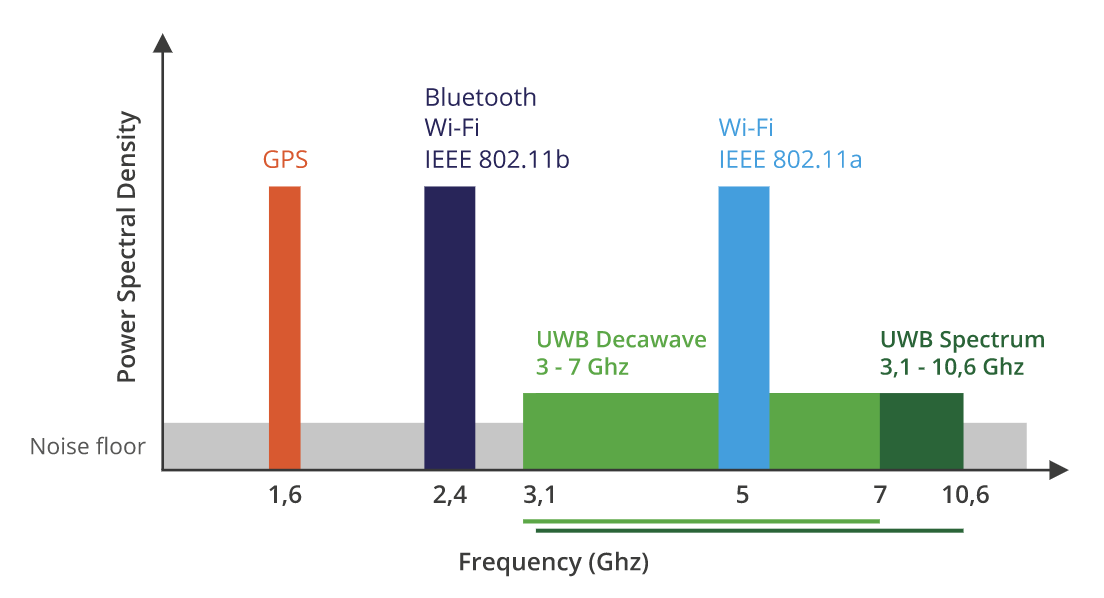
\includegraphics[width=.6\linewidth]{Images/uwb_bandwidth.png}
\centering
\caption{UWB spectrum compared to Wi-Fi and other wireless technology. Taken from \cite{itur2006characteristics}.}
\label{fig:UWB_Techonology}
\end{figure} 

Knowing this and based on the time-frequency duality reminded in eq. \ref{fig:eq}, one can see that the extension in the time domain will be quite small compared to other signals type. This is a direct effect of the Fourier transform, the extension of a function and it's extension of it's Fourier transform are inversely proportional. This follows the principle of uncertainty assessing that a trade-off needs to be done between the precision reached in the time domain and the one in the frequency domain \cite{donoho1989uncertainty}.

\begin{equation}
	x(at) \longleftrightarrow \frac{1}{|a|}*X(\frac{f}{a})
\label{fig:eq}
\end{equation}

The Fig. \ref{fig:UWB_time} shows the theoretical duration of an impulse of the \gls{uwb}. One can see that the time extension of the significant part of the pulse is from 0.3 to 0.7 nanoseconds, leading to a pulse duration of 0.4 nanoseconds.

\begin{figure}[H]
\centering
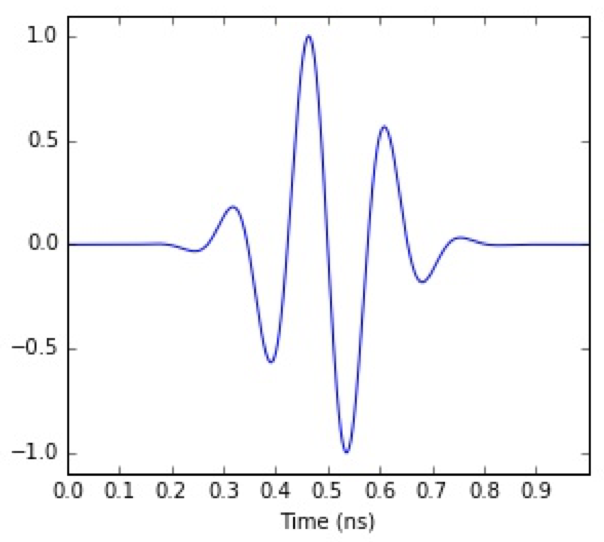
\includegraphics[width=.4\linewidth]{Images/uwb_pulse.png}
\caption{Theoritical duration of an UWB pulse. Taken from \cite{defraye2017determining}.}
\label{fig:UWB_time}
\end{figure}

An advantage of the \gls{uwb} is its robustness in regard of the \glspl{mpc} \color{red} EXPLIQUER CE QUE SONT LES MPCS \color{black}.  This can be understood by looking at Fig. \ref{fig:UWB_MPC_Theo}, where several peaks can be distinguished, each corresponding to a different path travelled by the wave. Indeed, the probability to have a collision depends on the size of the pulse sent. From this, the interest of the \gls{uwb} in confined area appears as a lot of \gls{mpc} are present due to the reflections coming from all walls of a room.

\begin{figure}[H]
\centering
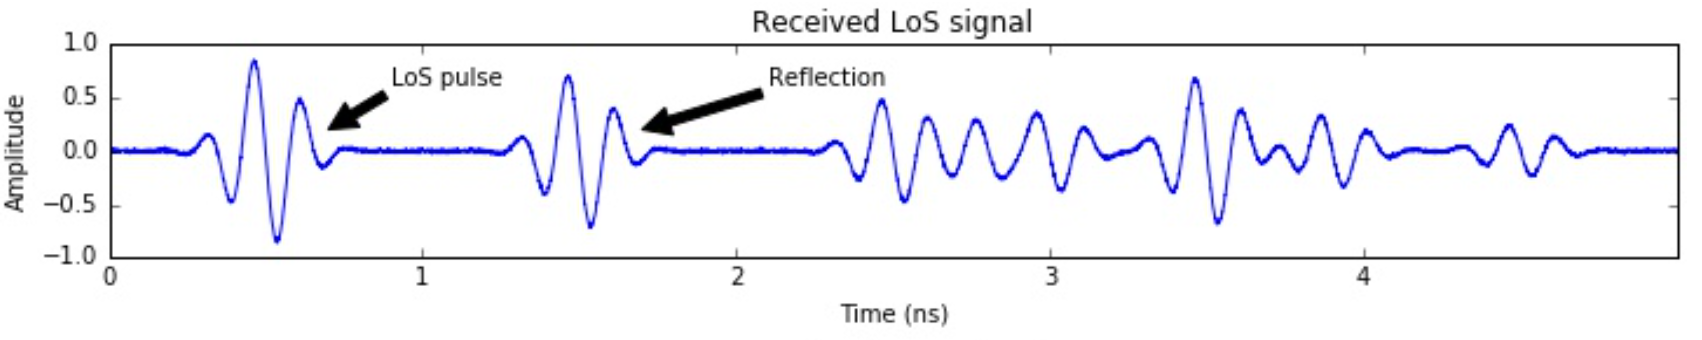
\includegraphics[width=.9\linewidth]{Images/mpc_pulses.png}
\caption{Example of an MPC with a \gls{los} and a \gls{nlos}. Taken from \cite{defraye2017determining}\color{red} DEFINIR LOS ET NLOS \color{black}}
\label{fig:UWB_MPC_Theo}
\end{figure}

\section{Real Time Locating Systems}
\label{rtls}
\gls{rtls} are systems used to track and identify the location of objects in real time. This is a rather vague definition since nothing is specified concerning the means employed to achieve the localization. The \gls{rtls} that will be presented in this section will all have in common the use of wireless communications, between devices called "anchor" and "tag", the tag being associated with the object to locate while the anchor is at a fixed and known location.
\vspace{2mm}

Those \gls{rtls} can be separated in two categories : "Relative localization" and "Absolute localization". The relative localization algorithm presented in section \ref{sds2wr} is the \gls{tof} method that is used in this project to compute the distance between an anchor and a tag. This choice has been made and explained in \cite{fesler2018high}, \cite{hannotier2019indoor} alongside a presentation of several approaches to determine the relative position of a tag relatively to an anchor. \color{red} Detailler plus cette partie \color{black}

\subsection{Symmetric double sided two-way ranging}
\label{sds2wr}

\gls{sdstwr} consists in an exchange of three messages between two \glspl{rdev}, respectively '$RDEV_1$' initiating the communication and '$RDEV_2$'. Each device needs to save the \gls{toe} or \gls{toa} of every message. Those times being respectively $t_0$, $t_1$ for the first message, $t_2$, $t_3$ for the second message and $t_4$, $t_5$ for the last message.
\vspace{2mm}

Each message contains the different timestamps previously computed, meaning that at the end of this exchange $RDEV_2$ possess all the informations about the timestamps, while $RDEV_1$ misses the last one. If one wants $RDEV_1$ to be able to compute the \gls{tof} then a last message containing $t_5$ should be exchanged.
\vspace{2mm}

A schematic of the exchanges between $RDEV_1$ and $RDEV_2$ that occurs in \gls{sdstwr} is shown in Fig. \ref{sdstwr}. 

\begin{figure}[H]
\centering
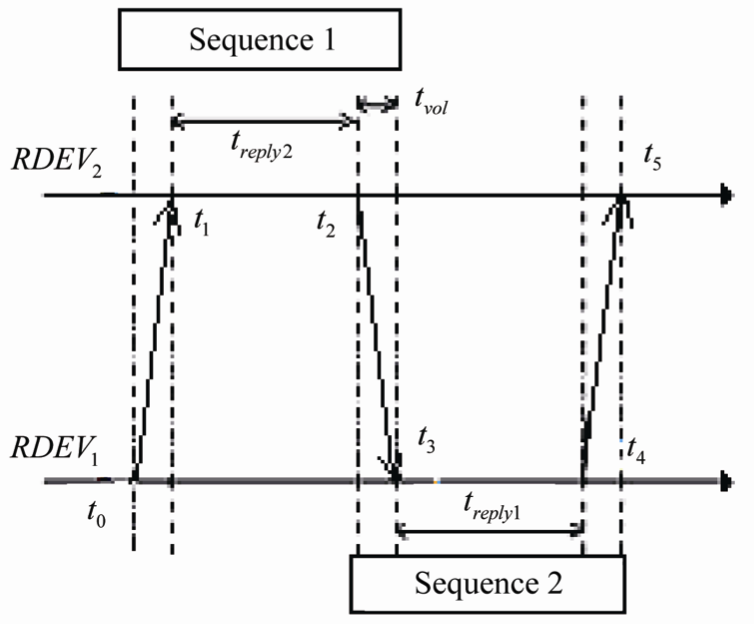
\includegraphics[width=.6\linewidth]{Images/sds-twr.png}
\caption{Symmetric double-sided two-way ranging. Taken from \cite{dalce2011comparison}.}
\label{sdstwr}
\end{figure}

Based on those timestamps, the computation of the \gls{tof} can be observed in eq. \ref{fig:tof}. This estimation is the arithmetic means of the \gls{tof} from '$RDEV_1$' to '$RDEV_2$' and vice-versa.

\begin{equation}
	t_{est} = \frac{((t_3 - t_0) - (t_2 - t_1)) + ((t_5 - t_2) - (t_4 - t_3))}{4}
\label{fig:tof}
\end{equation}

Since that \gls{tof} computed remains an estimation, it is important to know the magnitude of the error as well as its evolution in parallel of the true value of the \gls{tof}.

\begin{equation}
	t_{true} - t_{est} = \frac{1}{4}*((t_2 - t_1) - (t_4 - t_3))*(e_1 - e_2)
\end{equation}

The term $e_1 - e_2$ being the difference between the internal clocks of both devices. \cite{dalce2011comparison}

\subsection{Trilateration}
\label{tril}

The \gls{sdstwr} allowing us to compute the \gls{tof}, the relative distance can be computed using the light celerity. If the relative distance between a tag and three different anchors is known, it is possible to compute the intersection of three circle having as center the position of the anchor and radius corresponding to the \gls{tof} associated to this anchor. A scheme displaying that solution can be seen on Fig. \ref{fig:trilateration}.

\begin{figure}[H]
\centering
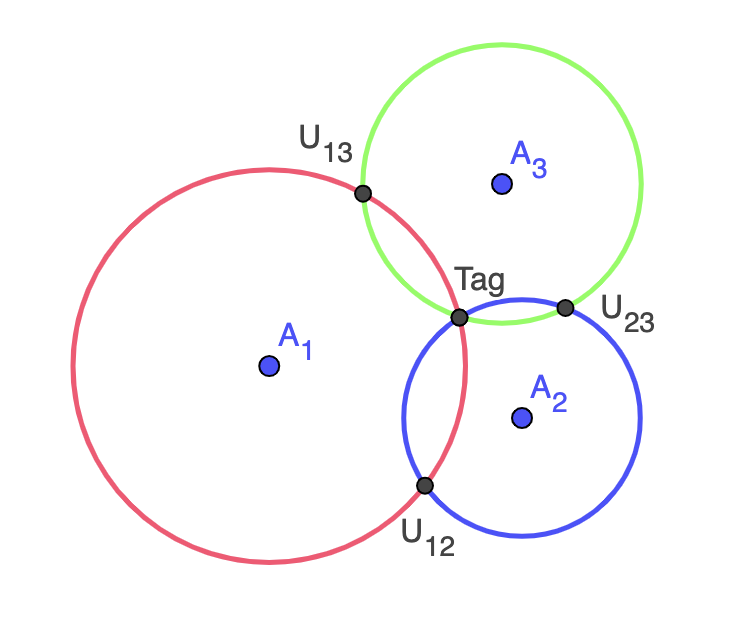
\includegraphics[width=.5\linewidth]{Images/trilateration.png}
\caption{Trilateration \label{fig:trilateration}}
\end{figure}

As one can deduce, in a two dimensional  plan, three anchors are needed to have an intersection of only one point, removing the uncertainty on the solution. If only two anchors where used, one would obtain two possible solution : $Tag$ and $U_{XY}$. In a three dimensional space, four anchors would be needed. This actually corresponds to 
the following system of equations :

\begin{equation}
\label{eq:syst_exact}
\begin{cases}
(x_1 - x_0)^2 + (y_1 - y_0)^2 = d_1^2 \\
(x_2 - x_0)^2 + (y_2 - y_0)^2 = d_2^2 \\
(x_3 - x_0)^2 + (y_3 - y_0)^2 = d_3^2 \\
\end{cases}
\end{equation}

Where $(x_i, y_i)$ corresponds to the position of the anchor $i$ and $d_i$ corresponds to the distance between this anchor and the tag, $(x_0, y_0)$ being the position of the tag.

\subsubsection{Uncertainties}

Due to the inaccuracy of the computed distances, the system \ref{eq:syst_exact} can not be solved. There is a lot of probability that there is not a single point $(x_0, y_0)$ that solves it. To avoid this problem, the estimator $S(\vec{p})$ developed in \cite{zhou2009efficient} is used.

\begin{equation}
\label{eq:syst_approx}
\begin{aligned}
S(\vec{p_0}) &= \sum_i^N (\|\vec{p_i} - \vec{p_0}\| ^2 - d_i^2 )^2 \\
\vec{p_0} &= \underset{\vec{p}}{\text{argmin}}~ S(\vec{p})
\end{aligned}
\end{equation}

Where $\vec{p_k} = (x_k, y_k) \forall k\in {0, ... , N}$ in the two dimensional cases, N being the number of anchors\footnote{Which can be superior to 3, even in a 2D plan.}. The objective of this estimator is to find the estimate $\vec{p_0}$ minimizing the value of $S(\vec{p_0})$.
% Rappeler le concept avec un schéma concis. 

\section{Implementation of a locating system}
\label{loc_syst}

Using the technology briefly presented in sections \ref{uwb} and \ref{rtls}, a locating system has been developed by Quentin Fesler and Cédric Hannotier in  \cite{fesler2018high}, \cite{hannotier2019indoor}. This system is able to retrieve a localization with an error oscillating between twenty and fifty centimetres inside of a building \cite{guyard2019navigation}.
\vspace{2mm}

This locating system is composed of fixed antennas called anchors, based on ESP8266 as micro-controller and a Decawave DWM1000 \gls{uwb} transceiver\cite{decawave}. The tag are built using an Android cellphone, a PSoC\footnote{The exact model is the : CY8C5888LTI-LP097 \cite{guyard2019navigation}.} and also a DWM1000 module.

\subsection{DWM1000}
\label{dwm1000}

The DWM1000 is the antenna chosen to operate the wireless communication, it will be needed for the tag as well as for the different anchors. The configuration of those antennas and the \gls{spi} communication are both explained in this section.

\begin{figure}[H]
	\centering
	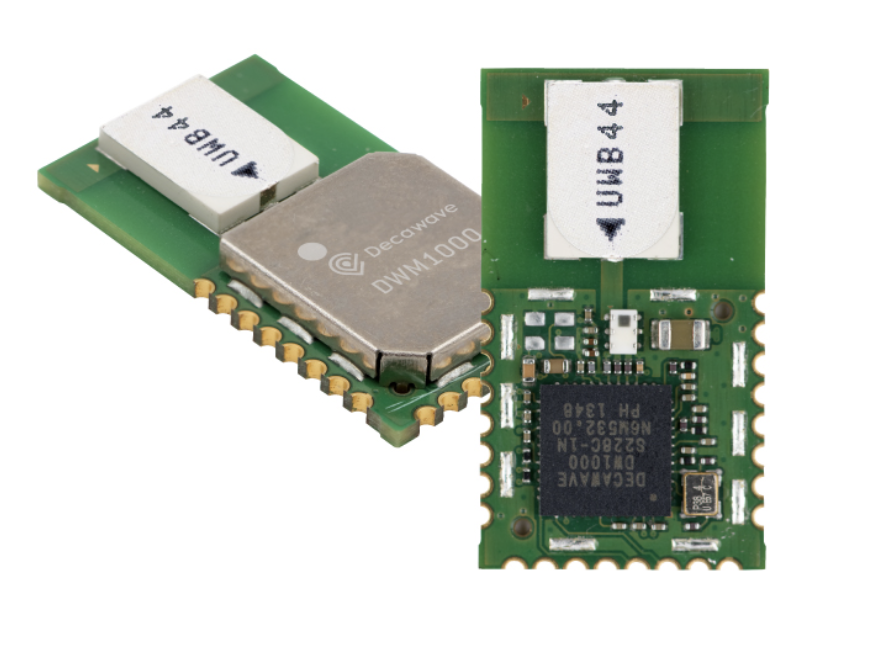
\includegraphics[width=.3\linewidth]{Images/DWM1000.png}
	\label{fig:dwm1000}
	\caption{DWM1000 module. Taken from \cite{decawave}.}
\end{figure}

\subsubsection{Configuration}

Before using the DWM1000, tests have been conducted to choose a configuration minimizing the error rate and the consumption while maximizing the communication speed. This leads to the following choices\footnote{A more detailed discussion on the choice of those parameters can be found in \cite{hannotier2019indoor}.} :

\begin{itemize}
\item Channel number : 5
\item Bitrate : 6.8 Mbits\textsuperscript{-1}
\item \gls{prf} : 16MHz
\item Preamble length : 128 bits
\end{itemize}

The chosen channel number is the number 5 partly due to the \gls{eu} regulations that are more strict in the frequencies bounds from 3.1 to 4.8 GHz than in the frequencies bounds from 6 to 9 GHz\cite{eulaw}. The other channel that is in those more  boundaries in the $7^{th}$ one. The difference being a bandwidth being twice as largei\footnote{The bandwidth of the $5^{th}$ one is 499.2MHz while the one from the $7^{th}$ is 1081.6 MHz.}. The channel 7 also lies within this region of the electromagnetic spectrum, but was not chosen. The difference between those channel resides in the size of the bandwidth.
\vspace{2mm}

The choices of the bitrate are restricted between 110 kbits\textsuperscript{-1}, 850 kbits\textsuperscript{-1} or 6800 kbits\textsuperscript{-1}. The reasons behind the choice of the bitrate at 6.8 Mbits\textsuperscript{-1} are detailed in \cite{hannotier2019indoor}. This principal reason being the existence of a "Smart Transmit Power Control" allowing to increase the power of transmission under certain conditions, one of them being that the bitrate must be fixed at 6.8 Mbits\textsuperscript{-1}.
\vspace{2mm}

The \gls{prf} can be chosen between 16 MHz and 64 MHz, an higher one increasing the operating range while consuming more power.
\vspace{2mm}

The preamble length is used to estimate the channel estimation, which describes how a signal propagates from the transmitter to the receiver, in order to perform the equalization to flatten the frequency response. The precision of the estimation increases with the size of the preamble. Unfortunately, a longer preamble means that a larger proportion of the energy consumed will not be used effectively, thus decreasing the energy efficiency of the setup, and that a shorter time window will be available to transmit actual data.  Recommended bitrate in function of the channel are proposed in \cite{usermanual}.
\vspace{2mm}

\subsubsection{Control}

The DWM1000 is piloted via an \gls{spi} bus, this communication follows a master-slave scheme where the master, which is the micro-controller, controls the communication \cite{busspi}. On Fig. \ref{fig:spi_scheme}, the four needed signals are displayed. \gls{miso} and \gls{mosi} are the connections used to transmit the data between the master and its slave. The \gls{sckl}, generated by the master fixes the speed at which the MISO and MOSI exchanges data. Since the \gls{spi} allows different slaves for only one master, the \gls{ss} is used by the master to select with which specific slave it communicates. 

\begin{figure}[H]
	\centering
	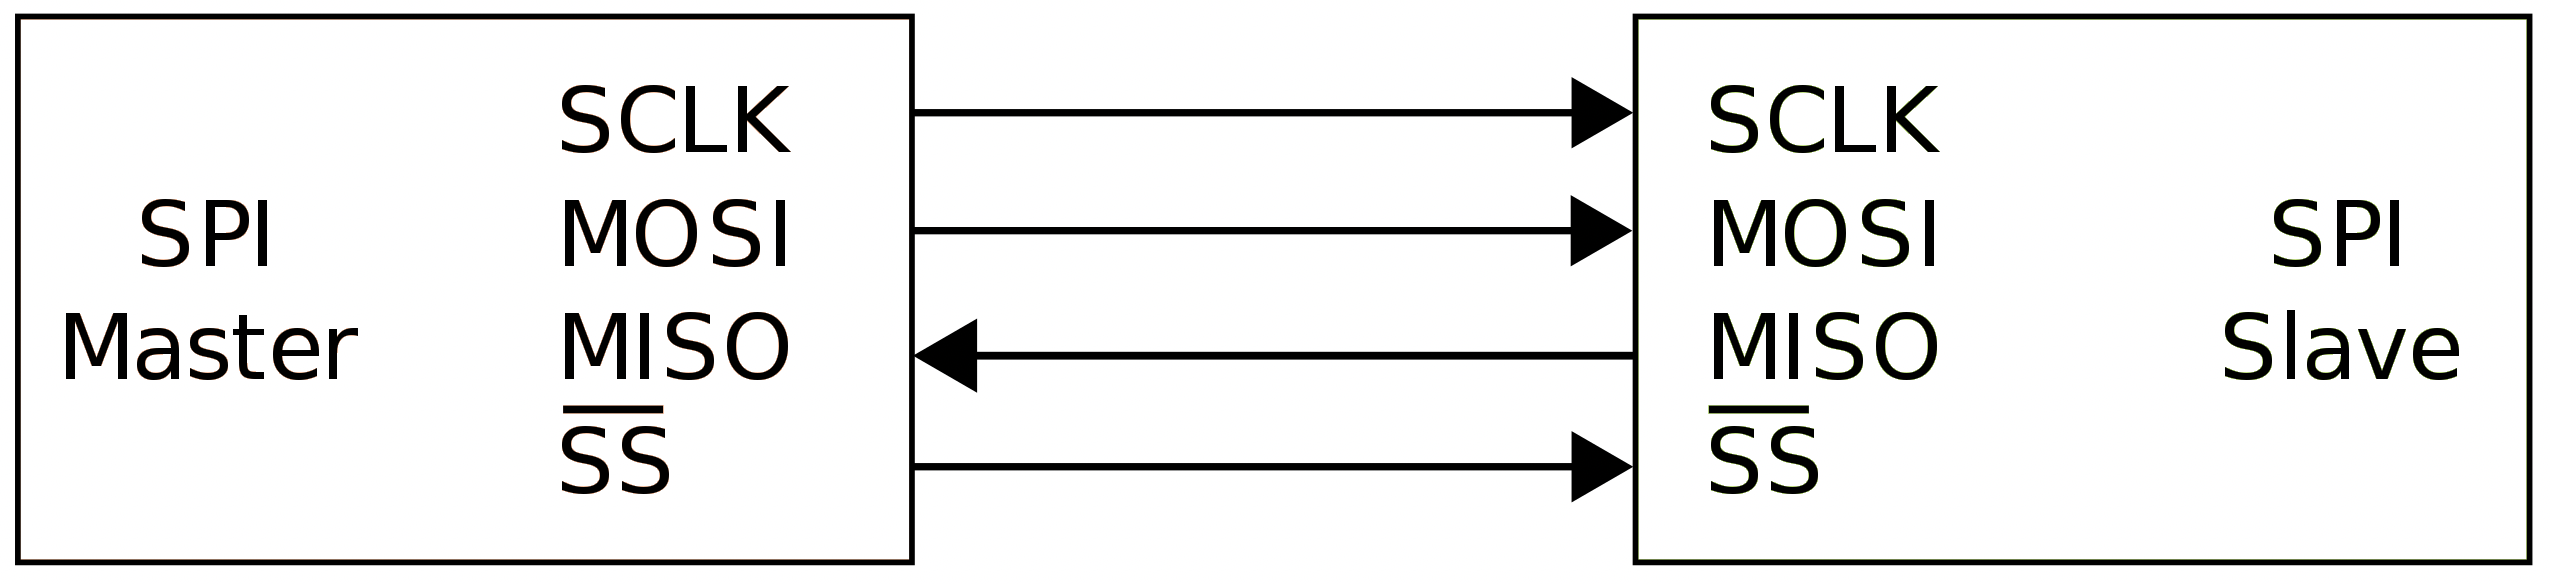
\includegraphics[width=.6\linewidth]{Images/SPI_scheme.png}
	\caption{SPI Schematic.}
	\label{fig:spi_scheme}
\end{figure}

\subsection{Anchor}

The anchors are fixed antennas composed of a DWM1000 and an ESP8266 \cite{esp8266}. They are placed at known position in the room and are used to compute the \gls{tof} between them and the tag using the \gls{sdstwr}, as explained in section \ref{sds2wr}. 

\begin{figure}[H]
	\centering
	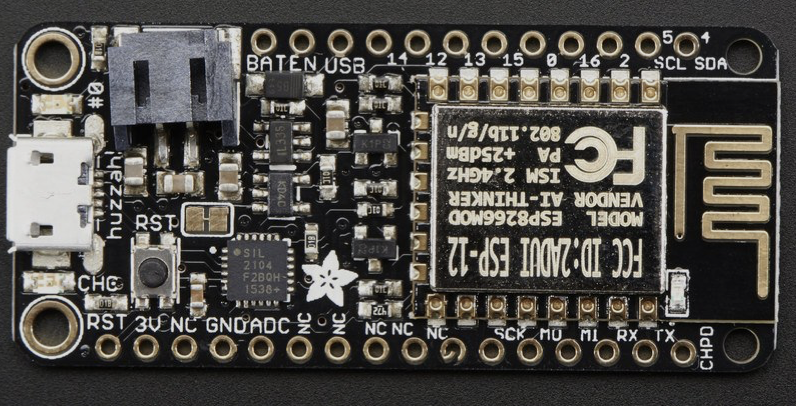
\includegraphics[width=.6\linewidth]{Images/esp8266.png}
	\caption{ESP8266 mounted on a Feather Huzzah board. Taken from \cite{adafruit}}
	\label{fig:esp8266}
\end{figure}

The micro-controller has been combined with the development board Feather Huzzah from Adafruit \cite{adafruit}. This module is represented in Fig. \ref{fig:esp8266}. This board can be flashed using a USB serie connection, allowing a easy deployment of the code. It also has the advantage of being light and small, a feature which is useful when one wants to deploy several anchors in a room. 

\subsection{Tag}

The tag is the object whose localization has to be determined. It is composed of a DWM1000 antenna, a PSoC\footnote{The exact model is the CY8C5888LTI-LP097 \cite{guyard2019navigation}.} and an Android application. The Fig. \ref{fig:psoc} shows the PSoC used as well as its custom board made by the electronic BEAMS service of the ULB.
\vspace{2mm}

\begin{figure}[H]
	\centering
	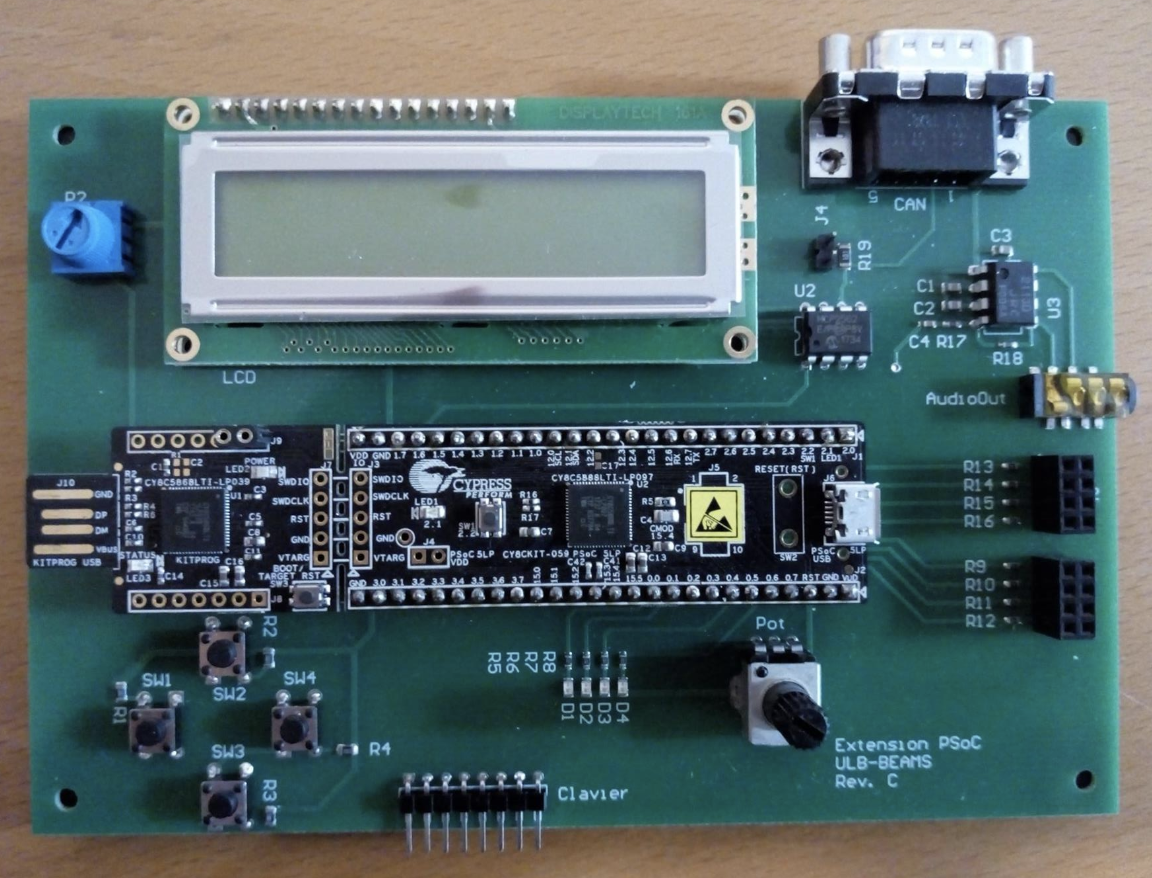
\includegraphics[width=.55\linewidth]{Images/psoc.png}
	\caption{PSoC micro-controller mounted on a custom board made by the BEAMS service.}
	\label{fig:psoc}
\end{figure}

The communication between the DWM1000 an the PSoC is performed using a \gls{spi} bus as for the anchors, the PSoC being the master. As for the ESP8266, the PSoC can be flashed through an USB bus. The micro-controller receives instructions from the application on the cellphone and controls the communications of the DWM1000 with the different anchors. It then transmits the received data from the DWM1000 to the application through an USB bus.

\subsection{Android Application}

To control the PSoC, an Android application has been developed. A screen-shot of the main window can be seen in the appendix \ref{app:app_view}. It exhibits four buttons, whose functionalities are presented in what follows.

\subsubsection{Navigation}

The Navigation button opens a map of an environment\footnote{The room UA5.214 in this case, which is one of the electronic lab at the ULB.} and an arrow is displayed at the estimated location of the tag, the orientation being the estimated orientation of the cellphone. The coordinates are also shown, computed from the bottom left corner of the map. The used map is shown in Fig. \ref{fig:ua5_map}.

\begin{figure}[H]
	\centering
	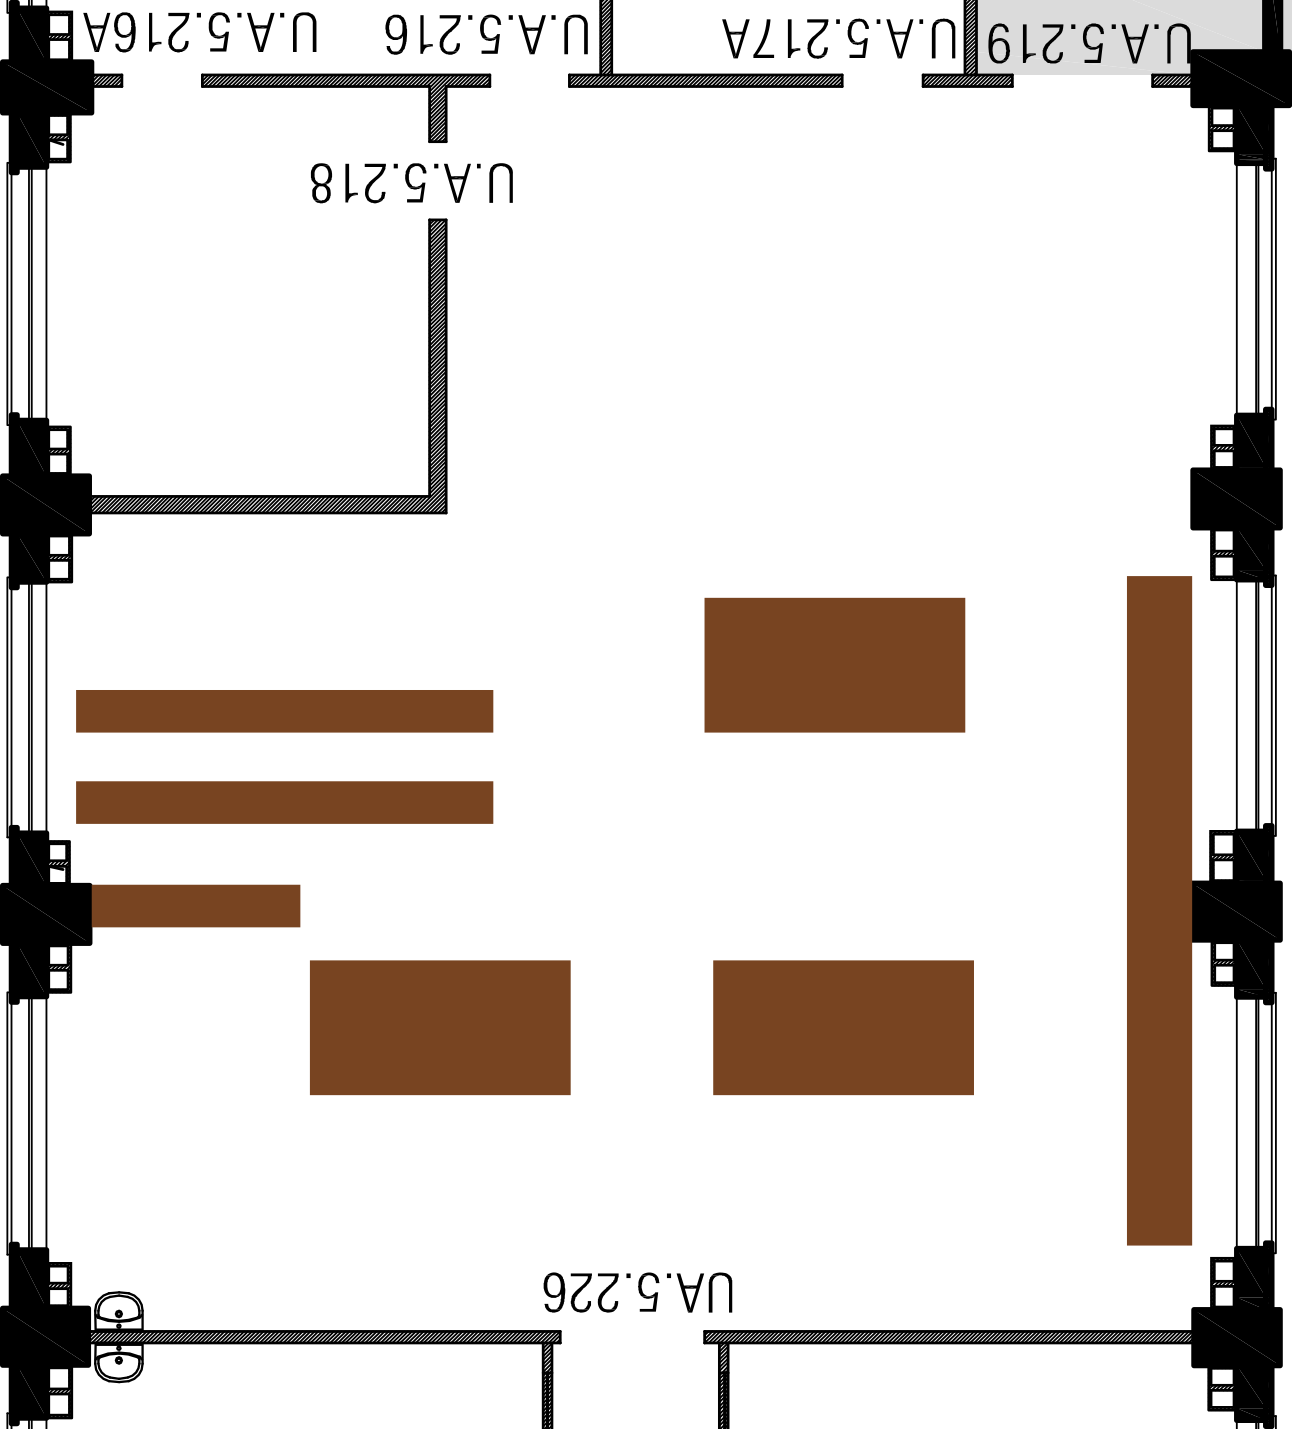
\includegraphics[width=.4\linewidth]{Images/little_room.png}
	\caption{Map of the UA5.214}
	\label{fig:ua5_map}
\end{figure}

When this function runs, the application enters a loop that continuously requests the PSoC to perform a \gls{sdstwr} with each anchor. The data containing the different timestamps are transmitted towards the application for each anchor separately. From those data, the distance between each anchor and the tag is computed on the cellphone as well as the trilateration algorithm described in section \ref{tril}, leading to an estimate of the location. The biggest computations are done on the cellphone because of the bigger computational power available in comparison to the PSoC.
\vspace{2mm}

A detailed state machine representing the interactions between the tag and an anchor can be found in appendix \color{red} make a link to an annex and put the state machine in annex \color{black}  \cite{hannotier2019indoor}. While the anchor only performs one \gls{sdstwr} at a time, the tag needs to keep an history of the anchors contacted to perform the trilateration afterwards.

\subsubsection{Test USB connection, Test orientation}

The Test USB connection allows to test that the USB communication bus used to communicate with the PSoC is fully operational. The test procedure consists of sending a 16 bits long messages to the PSoC, this message being : \texttt{0x0406}. If the PSoC is well connected, the application is supposed to receive a 32 bits long message : \texttt{0x02034637}. This feature allows to quickly debug the USB communication.
\vspace{2mm}

The "Test orientation" has been designed to test the detection of the orientation of the cellphone. The three angles necessary to characterize the orientation of the device are respectively the Azimuth, the Pitch and the Roll.

\begin{figure}[H]
\centering
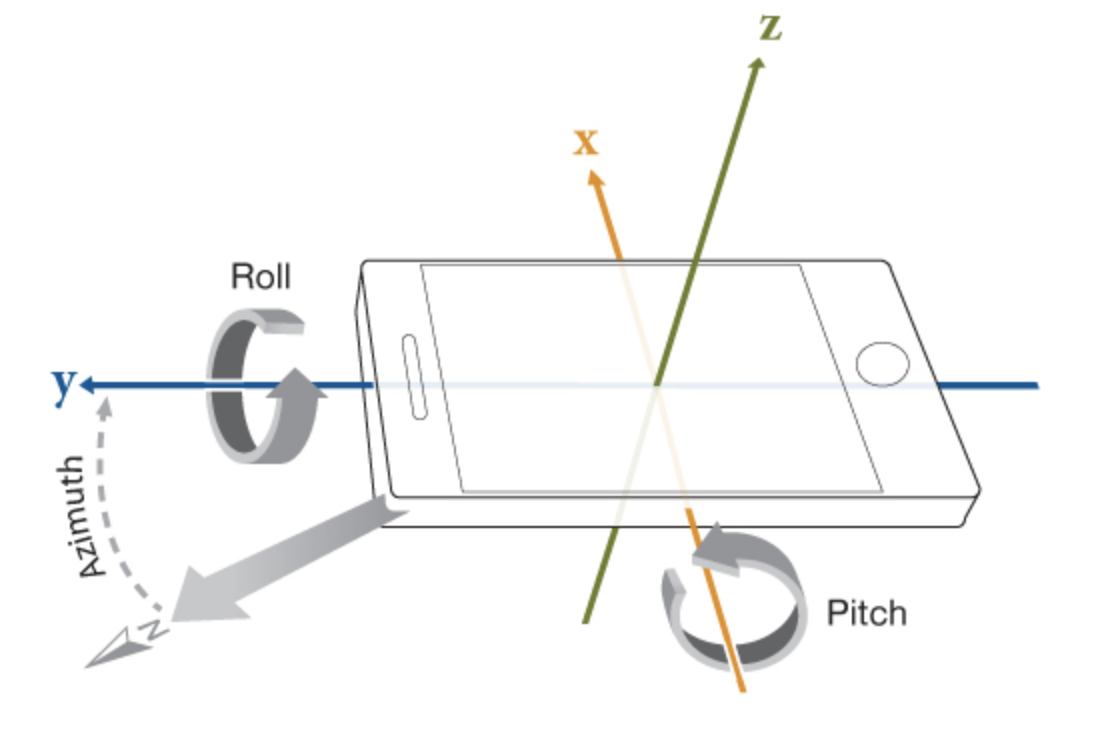
\includegraphics[width=.6\linewidth]{Images/angles_gsm.png}
\caption{Representation of the Roll, Pitch and Azimuth orientation parameters. Taken from \cite{mathworks}.}
\end{figure}

\subsubsection{Calibration}

The "Calibration" has been designed to enhance the precision on the timestamps. Indeed, there is a difference between the moment when the packet is received at the antenna of the DWM1000 and the moment of its detection, which corresponds to the timestamp. The same phenomena appears when the \gls{uwb} transceiver transmits a packet. Those errors on the timestamps are called the transmit/receive antenna delay and must be configured to match the actual antenna delay.

\color{red} Expliquer l'origine des delays \color{black}

\subsection{Precision obtained}

The precision obtained with this locating system depends on several factors, some of which being the location of the anchors in the room, the distance of the tag to those anchors, the clutter of the room, etc...
\vspace{2mm}

Nonetheless, a statistical study has been conducted to assess the performances of the locating system. The tag has been placed at several location that can be observed in Fig. \ref{fig:test_map}.

\begin{figure}[H]
	\centering
	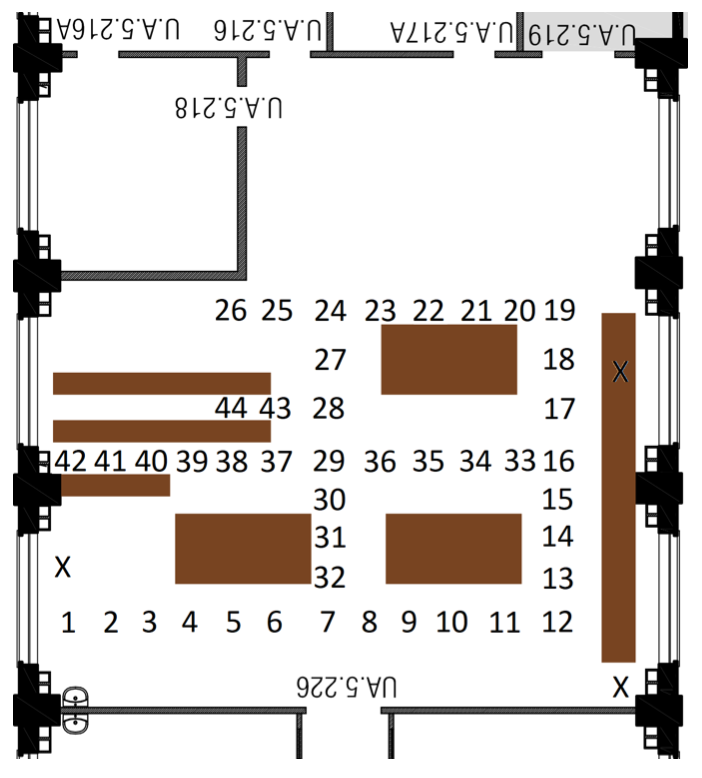
\includegraphics[width=.35\linewidth]{Images/test_map.png}
	\caption{Locations corresponding to the measures represented in Fig. \ref{fig:test_result}. Taken from \cite{hannotier2019indoor}.}
	\label{fig:test_map}
\end{figure}

For each location, the measurement was repeated a hundred times. The error remains below 45 cm for 80\% of the measurements but reaches up to 85 cm in the worst case. Such deviations can be explained by many different factors, among which the non-trivial geometry of the room, the walls that are not parallel, the presence of windows, ... \cite{hannotier2019indoor}. The extremity of the vertical segment represent the minimal and maximal errors for each locations.
\vspace{2mm}

\begin{figure}[H]
	\centering
	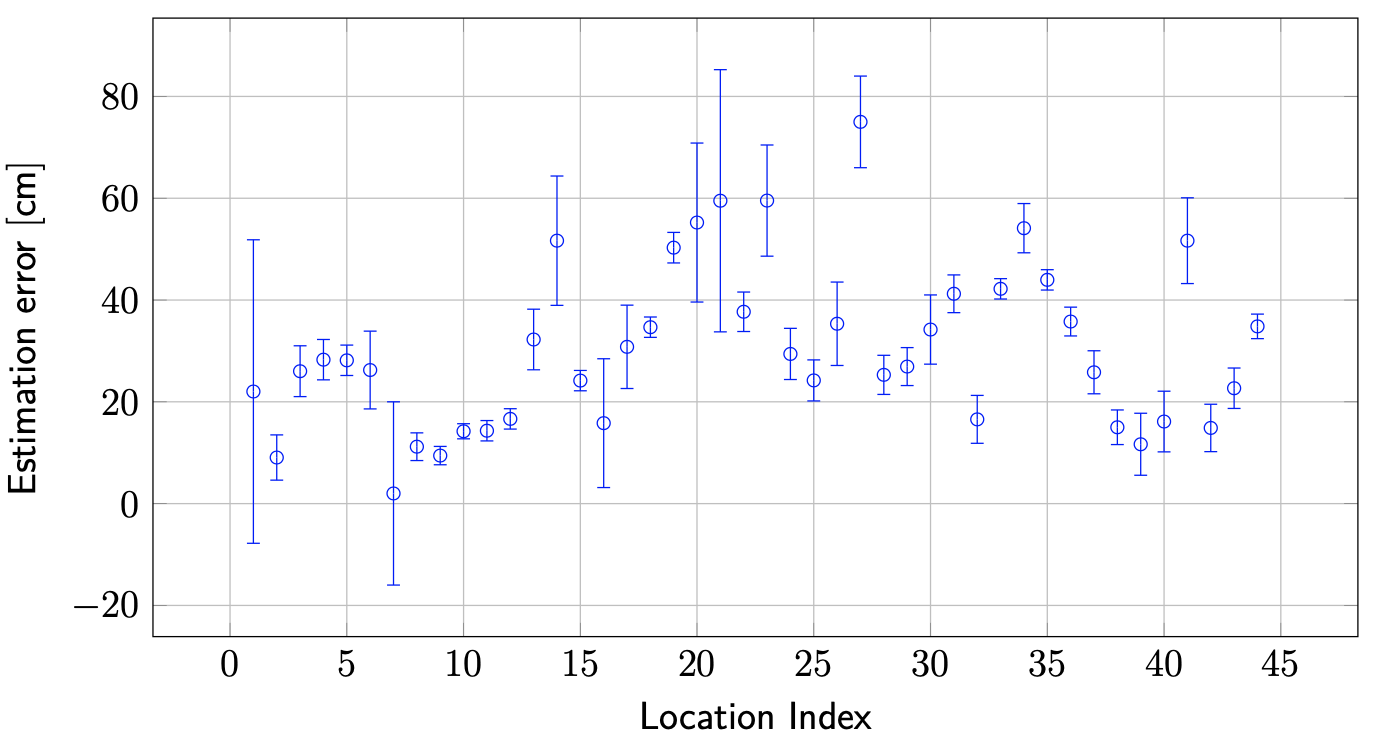
\includegraphics[width=.8\linewidth]{Images/test_fig.png}
	\caption{Error on the estimated location in function of the position of the tag. Taken from \cite{hannotier2019indoor}.}
	\label{fig:test_result}
\end{figure}

To achieve a better localization, anchors can be added. It has the advantage to add an equation to the system shown in eq. \ref{eq:syst_approx}, which, if the new anchor gives some coherent measure, improves the estimation of the localization. The drawback is that it will slow done the actualization of the position, since the tag has to communicate with more anchors. Such an algorithm dealing with four anchors is presented in \cite{guyard2019navigation}.

\section{Multi-path aided locating system}
\label{mpls}

\color{red} Rajouter un fil rouge du fonctionnement \color{black}

\subsection{Channel Impulse Response}
\label{mp_cir}

The \gls{cir} has already been mentioned in the section \ref{uwb}. The \gls{cir} is not only used in telecommunications systems but also in control theory for example, to characterize the behaviour of a system\footnote{In control theory, the transfer function which corresponds to the step response is commonly used.} \cite{garonne2019course}. As the name states, the goal of this \gls{cir} is to characterize the reaction of a system to a stimulus in the form of a pulse.
\vspace{2mm}

An example is displayed on the Fig. \ref{fig:cir_ex1}. A ray tracing has been performed on the left image. The \gls{los} rays and their first reflection can be observed. If a Dirac pulse is sent from the transmitter (TX) to the receiver (RX), since the propagation time will depend on the distance travelled, different peaks will appear, each corresponding to a different ray.

\begin{figure}[H]
	\centering
	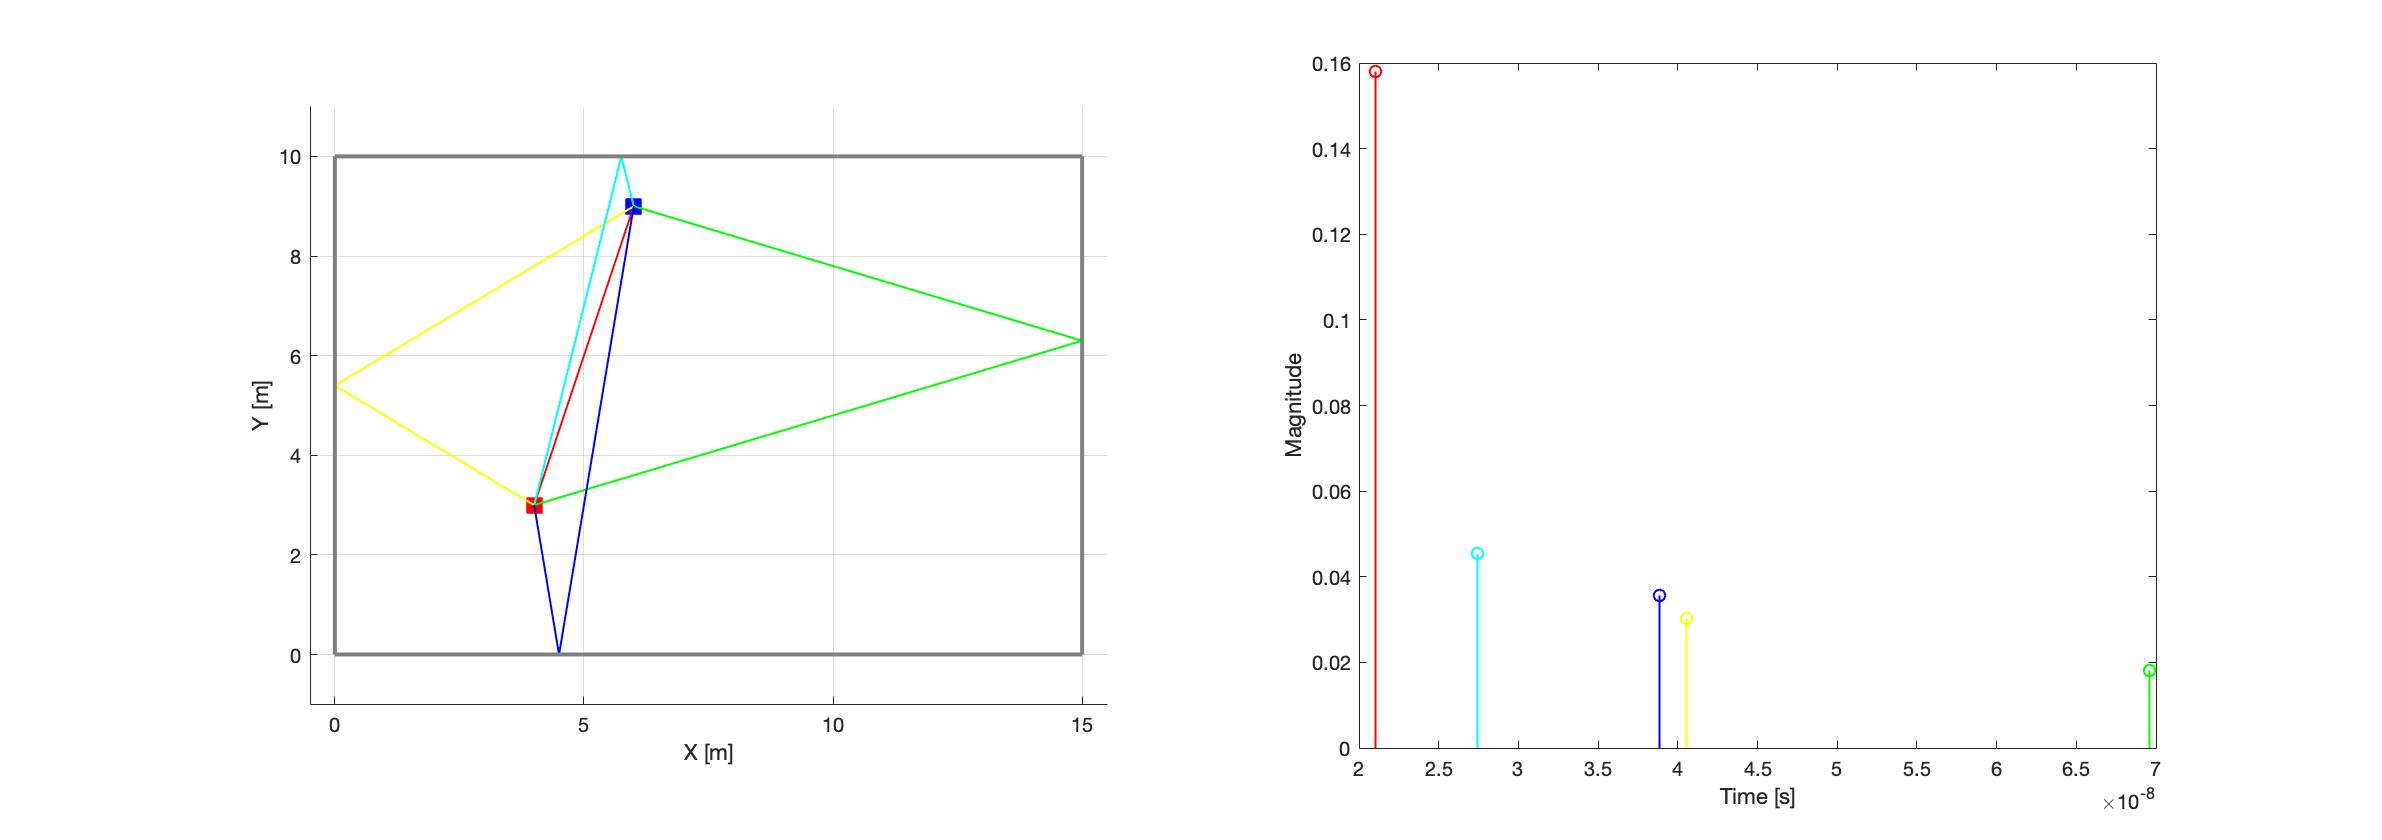
\includegraphics[width=.95\linewidth]{Images/Anchor-mpc.jpg}
	\caption{(Left) Direct and simple reflected rays between an anchor $(4, 3)$ and a tag $(6, 9)$. (Right) Theoretical CIR associated to each ray displayed in the map. 	\label{fig:cir_ex1}}

\end{figure}

As one can see, those different arrival times for each ray correspond to the different peaks on the right figure of the Fig. \ref{fig:cir_ex1}. The heights of the peaks depend on the attenuation due to the reflections on the walls. The equations used to compute those attenuations are detailed in the section \color{red} $ref\{SectionNotWrittenYet\}$ \color{black}. 

\subsection{Virtual Anchors}

The concept of \gls{va} has been introduced in  \cite{meissner2010uwb}. While the anchors are some actual devices, the \gls{va} are not physically implemented. In order to create them, one needs to know the location of an anchor in a room as well as the exact geometry of the room. In Fig. \ref{fig:va_room}, the \glspl{va} have been created using the method of images. To find the location of the \gls{va} 1, the left wall act as the symmetry axis for an axial symmetry. From this, it is possible to extend this method to two reflections, two axial symmetries on two different walls would be needed in that case.

\begin{figure}[H]
	\centering
	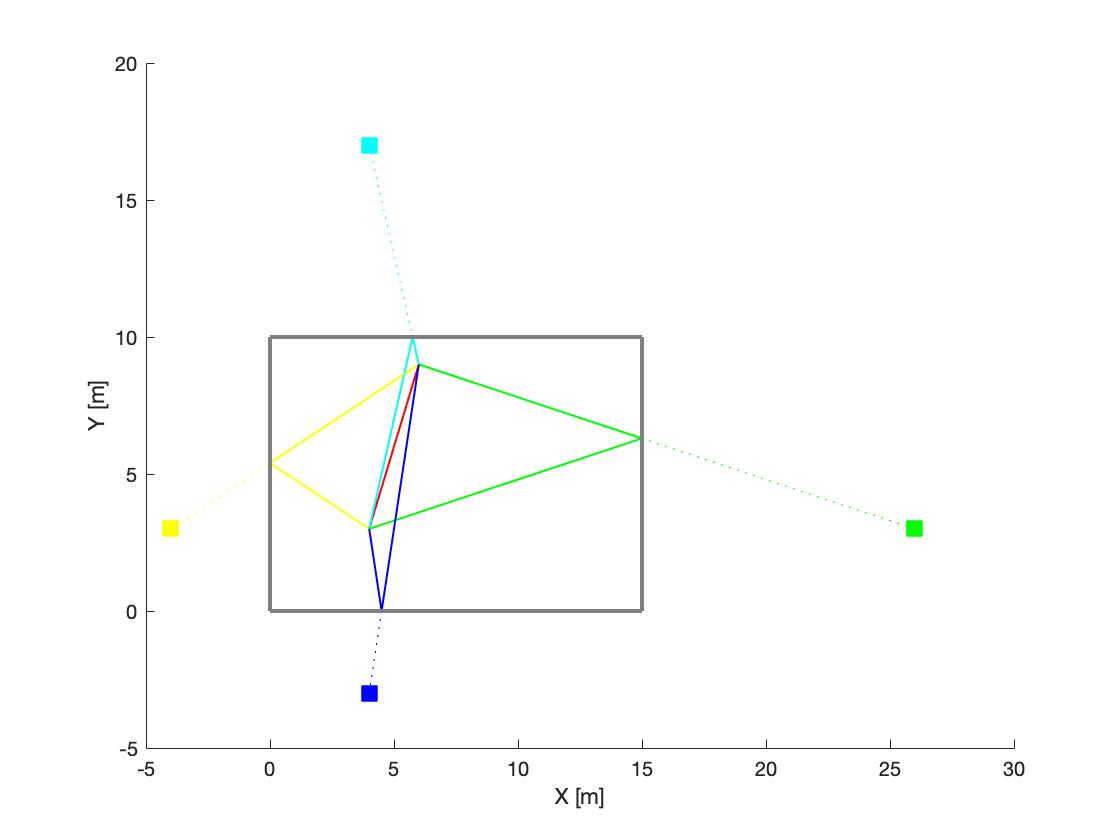
\includegraphics[width=.6\linewidth]{Images/va_map.jpg}
	\caption{VAs associated with its corresponding ray}
	\label{fig:va_room}
\end{figure}
 
Using the theoretical \gls{cir} from Fig. \ref{fig:cir_ex1}, each peak which is associated to a reflected ray can be considered as being the \gls{los} ray from a \gls{va} of Fig. \ref{fig:va_room}. The colors have been kept for the sake of clarity. The advantages of the methods of images is that the travelled distance by each ray as well as the angular distribution is kept unchanged.


\subsection{Locating system}
\label{loc_syst_mpc}

Based on the concept of \glspl{va} and \gls{cir}, several methods are proposed to find the localization of a tag in a room of known geometry using only one anchor.
\vspace{2mm}

In \cite{meissner2010mc}, the localization of a moving tag is proposed. This method uses the \gls{mpc} detected as well as the history of the position of the tag which allows to perform a cross-correlation with the newly detected position, therefore maximizing the coherence of the behaviour.
\vspace{2mm}

In \cite{froehle2013cooperative}, the \gls{comint} uses other tags in the room as anchor to perform the location. Each tag, acting as a transceiver and a receiver, communicates with the other tags to compute its distance relatively to those tag. An algorithm is presented in this paper that combines those different informations to achieve the localization.
\vspace{2mm}

\color{red} A refaire d'ici \color{black}

In \cite{jespersen2018indoor}, a method providing the tag location without using a history of the previous locations is proposed. Using the \gls{cir}, several pulses are detected, being equivalent to the \gls{tof} computed in the multiple anchor locating system previously presented. Nonetheless, there is a significant difference between both cases. In this method, each \gls{tof} is not associated with an anchor (virtual or not). Without knowing the position of the tag, one can not attribute each peak to an anchor\footnote{An exception is done for the first peak, since the \gls{los} that originates from the physical anchor is assumed to be the shortest path.}.
\vspace{2mm}

Due to this difference, the system \ref{eq:syst_approx} needs to be solved multiple times. Depending on the number of peaks detected, permutations between each \gls{va} needs to be done to test all the possibilities. The objective is still to find the $p_0$ value that minimize the equation.



% La on attaque la partie dure. Parler des ancres virtuelles, introduire le concept avec des schémas, montrer qu'on à dès lors besoin de la CIR.
% Parler des articles qui expliquent la théorie avec du MPC.